\def\DraftMode {false}

%%%%%%%%%%%%%%%%%%%%%%%%%%%%%%%%%%%%%%%%%%%%%%%%%%%%%%%%%%%%%%%%%%%%%%%%%%%%%%%%%%
%%%%%%%%%%%%%%%%%%%%%%%%%%%%%%%%%%%%%%%%%%%%%%%%%%%%%%%%%%%%%%%%%%%%%%%%%%%%%%%%%%
% packages

%\usepackage{german}
%\usepackage[ngerman,english]{babel}
%\usepackage[ansinew]{inputenc}
%\usepackage{subfigure}
\usepackage{pict2e}
\usepackage{epic}
\usepackage{amsmath,amsfonts,amssymb}
\usepackage{units}
\usepackage{fancybox}
\usepackage[absolute,overlay]{textpos} 
%\usepackage{tikz}
\usepackage{ifthen}
\usepackage{animate}
\ifthenelse{\equal{\DraftMode}{true}}{
\usepackage[draft]{media9}
}{
\usepackage{media9} % avi2flv: "C:\Program Files\ffmpeg\bin\ffmpeg.exe" -i TuneFreqFilterbank.avi -b 600k -s 441x324 -r 15 -acodec copy TuneFreqFilterbank.flv
}

%%%%%%%%%%%%%%%%%%%%%%%%%%%%%%%%%%%%%%%%%%%%%%%%%%%%%%%%%%%%%%%%%%%%%%%%%%%%%%%%%%
%%%%%%%%%%%%%%%%%%%%%%%%%%%%%%%%%%%%%%%%%%%%%%%%%%%%%%%%%%%%%%%%%%%%%%%%%%%%%%%%%%
% relative paths

\def\AcaGraph			{../../AudioContentAnalysis/graph}
\def\AcaTables			{../../AudioContentAnalysis/tables}
\def\AcaPict			{../../AudioContentAnalysis/picture}
\def\AcaEq				{../../AudioContentAnalysis/eq}

%%%%%%%%%%%%%%%%%%%%%%%%%%%%%%%%%%%%%%%%%%%%%%%%%%%%%%%%%%%%%%%%%%%%%%%%%%%%%%%%%%
%%%%%%%%%%%%%%%%%%%%%%%%%%%%%%%%%%%%%%%%%%%%%%%%%%%%%%%%%%%%%%%%%%%%%%%%%%%%%%%%%%
% counters, definitions, and commands

%---------------------------------------------------------------------------------
% colors
\definecolor{gtgold}{HTML}{E0AA0F} %{rgb}{0.88,0.66,1,0.06} [234, 170, 0]/256

%---------------------------------------------------------------------------------
% counters
\newcounter{i}
\newcounter{iXOffset}
\newcounter{iYOffset}
\newcounter{iXBlockSize}
\newcounter{iYBlockSize}
\newcounter{iYBlockSizeDiv2}
\newcounter{iDistance}

%---------------------------------------------------------------------------------
% math
\DeclareMathOperator*{\argmax}{argmax}
\DeclareMathOperator*{\argmin}{argmin}
\DeclareMathOperator*{\atan}{atan}
\DeclareMathOperator*{\arcsinh}{arcsinh}
\DeclareMathOperator*{\sign}{sign}
\DeclareMathOperator*{\tcdf}{tcdf}
\DeclareMathOperator*{\si}{sinc}
\DeclareMathOperator*{\princarg}{princarg}
\DeclareMathOperator*{\arccosh}{arccosh}
\DeclareMathOperator*{\hwr}{HWR}
\DeclareMathOperator*{\flip}{flip}
\DeclareMathOperator*{\sinc}{sinc}
\newcommand{\e}{{e}}
\newcommand{\jom}{\mathrm{j}\omega}
\newcommand{\jOm}{\mathrm{j}\Omega}
\newcommand   {\mat}[1]    		{\boldsymbol{\uppercase{#1}}}		%bold
\renewcommand {\vec}[1]    		{\boldsymbol{\lowercase{#1}}}		%bold

%---------------------------------------------------------------------------------
% media9
\newcommand{\includeaudio}[1]{\includemedia[
                        addresource=#1,
                        width=5mm,
                        height=5mm,
                        activate=onclick,
                        flashvars={
                            source=#1  
                            &autoPlay=true
                        }]
                        {
\includegraphics[width=5mm, height=5mm]{graph/SpeakerIcon}}
                        {APlayer.swf}}

\newcommand{\includevideo}[1]{\includemedia[
                        addresource=#1,
                        width=0.8\linewidth,
                        height=0.6\linewidth,
                        activate=onclick,
                        flashvars={
                            source=#1  
                            &autoPlay=true
                        }]
                        {}
                        {VPlayer.swf}}

%---------------------------------------------------------------------------------
% units
\setlength{\unitlength}{1mm}

%%%%%%%%%%%%%%%%%%%%%%%%%%%%%%%%%%%%%%%%%%%%%%%%%%%%%%%%%%%%%%%%%%%%%%%%%%%%%%%%%%
%%%%%%%%%%%%%%%%%%%%%%%%%%%%%%%%%%%%%%%%%%%%%%%%%%%%%%%%%%%%%%%%%%%%%%%%%%%%%%%%%%
% theme & layout
\usetheme{Frankfurt}

%---------------------------------------------------------------------------------
% fontsize
\let\Tiny=\tiny

%---------------------------------------------------------------------------------
% tocs
\setcounter{tocdepth}{1}
\AtBeginSection[]
{
    \begin{frame}<beamer>{overview}{~}
        \tableofcontents[currentsection]
    \end{frame}
}
% breadcrumbs - instead of one bullet per slide, do one per subsection
\useoutertheme[subsection=false]{miniframes}
\usepackage{etoolbox}
\makeatletter
\patchcmd{\slideentry}{\advance\beamer@xpos by1\relax}{}{}{}
\def\beamer@subsectionentry#1#2#3#4#5{\advance\beamer@xpos by1\relax}%
\makeatother

%---------------------------------------------------------------------------------
% appearance
\setbeamercolor{structure}{fg=gtgold}
\setbeamercovered{transparent} %invisible

%---------------------------------------------------------------------------------
% logo
\addtobeamertemplate{frametitle}{}{%
\begin{textblock*}{100mm}(8.3cm,.65cm)
\includegraphics[height=.8cm,keepaspectratio]{graph/CenterMusicTechnology-solid-2lines-white-CoAtag}
\end{textblock*}}

%%%%%%%%%%%%%%%%%%%%%%%%%%%%%%%%%%%%%%%%%%%%%%%%%%%%%%%%%%%%%%%%%%%%%%%%%%%%%%%%%%
%%%%%%%%%%%%%%%%%%%%%%%%%%%%%%%%%%%%%%%%%%%%%%%%%%%%%%%%%%%%%%%%%%%%%%%%%%%%%%%%%%
% title information
\title[]{Music DSP}   
\subtitle{MUSI 6202}
\author[alexander lerch]{alexander lerch} 
%\institute{~}
%\date[Alexander Lerch]{}
\titlegraphic{\vspace{-16mm}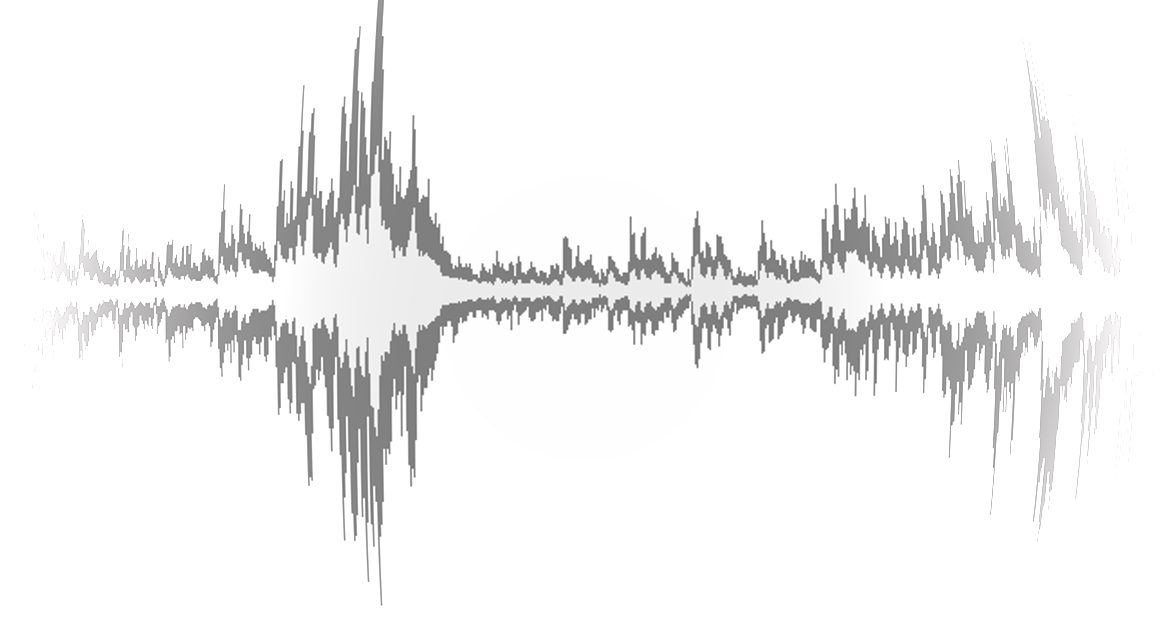
\includegraphics[scale=.25]{graph/title}}
